\section{Timing analysis} 

During recent years it was found that a lot of information about an X-ray binary could be obtained with its luminosity timing properties.
Very first one could examine luminosity variability power spectrum, which typically can be represented with the set of broad and thin Lorentzian functions representing correspondingly Fourier continuum and QPOs \citep[see, e.g.][]{1972ApJ...174L..35T, 1990A&A...227L..33B}.
It was found that variability properties changes with the system state - e.g. variability amplitude significantly lower in the soft state \citep{},  and also with the luminosity in particular state - for example position of some QPOs and the power spectrum break frequencies \cite{1990A&A...227L..33B}. 
Some aspects of the evolution of the XBs power spectrum with the system state can be explained in the frame of the accretion flow model with the geometrically thin cold disk and geometrically thick hot flow (corona), particularly it is widely accepted that the high amplitude variability is associated with the geometrically thick flow, while the geometrically thin disk is generally stable \citep{churazov}. 
It should be noted that this model of the variability generation are directly connected with the models, explaining energy spectra of black hole binaries \citep[see, e.g.,][]{1975ApJ...199L.153E, 1976ApJ...204..187S, 1995ApJ...452..710N}, \citet{churazov} has shown with the frequency resolved spectroscopy that variable part of the emission has a hard spectrum, which is thought to be produced in the corona, while stable part of the emission has a spectrum which is consistent with the cold classical $\alpha$-disc spectrum \citep{ss73}.

To explain the shape of the power spectra of the XBs different models were suggested. 
It is generally accepted that the broadband noise is produced in the coronal flow due to the stochastic variations of the angular momentum transport efficiency, \citep{lyubarskii97} model of the propagating fluctuations explains the shape of the luminosity variability power spectrum arising due to this process. 
There also a number of models, explaining high and low frequency QPO features in power spectra \citep[][]{ingram09, citesomething}. 
Most of that models were architect in order to explain energy spectra (or particular feature in it) and the power spectra. 
However, as will be discussed in the following chapter, additional analysis, describing time properties in different energy bands, can be applied to rule out some of that models.

\subsection{Power spectrum}
    The power spectra of each of the separate observation has a form of plateau ending on the frequency $\approx0.1$~Hz transforming in the power law with the slope $\rho\approx-2$ on the higher frequencies, it also contains a prominent QPO on the frequencies 0.3--0.7~Hz and second overtone, also there is clear Poisson noise component dominating over the source variability above $\sim2$~Hz.
    The shapes of the power spectra obtained from the light curves in different energy bands are very similar.
    In order to estimate QPO amplitude and location we fit Power Spectra with the following function:
\begin{equation}
        P(f) = n (1 + (f/f_{\rm lb})^4)^{\alpha} (1 + (f/f_{\rm hb})^4)^{\beta} + \frac{s_1}{(f - f_{qpo})^2 + (f_{\rm qpo} Q_{\rm m})^2} + \frac{s_2}{(f - 2f_{qpo})^2 + (f_{\rm qpo} Q_{\rm o})^2} + n_2 (1 + (f/f_{\rm vh})^2)^{\gamma} + poiss
        \label{eq:complex_fit}
\end{equation}
In this function first component represents plateau function with break, which can has complex shape (sharp or wide), second two components describe QPO main harmonics and its overtone, fourth component represents any additional high frequency power, it can be connected either with the detector dead time effects or can describe broad featureless component connected to the QPO power spreading to the high frequencies, last component represents constant Poisson noise component.

\begin{figure*}
        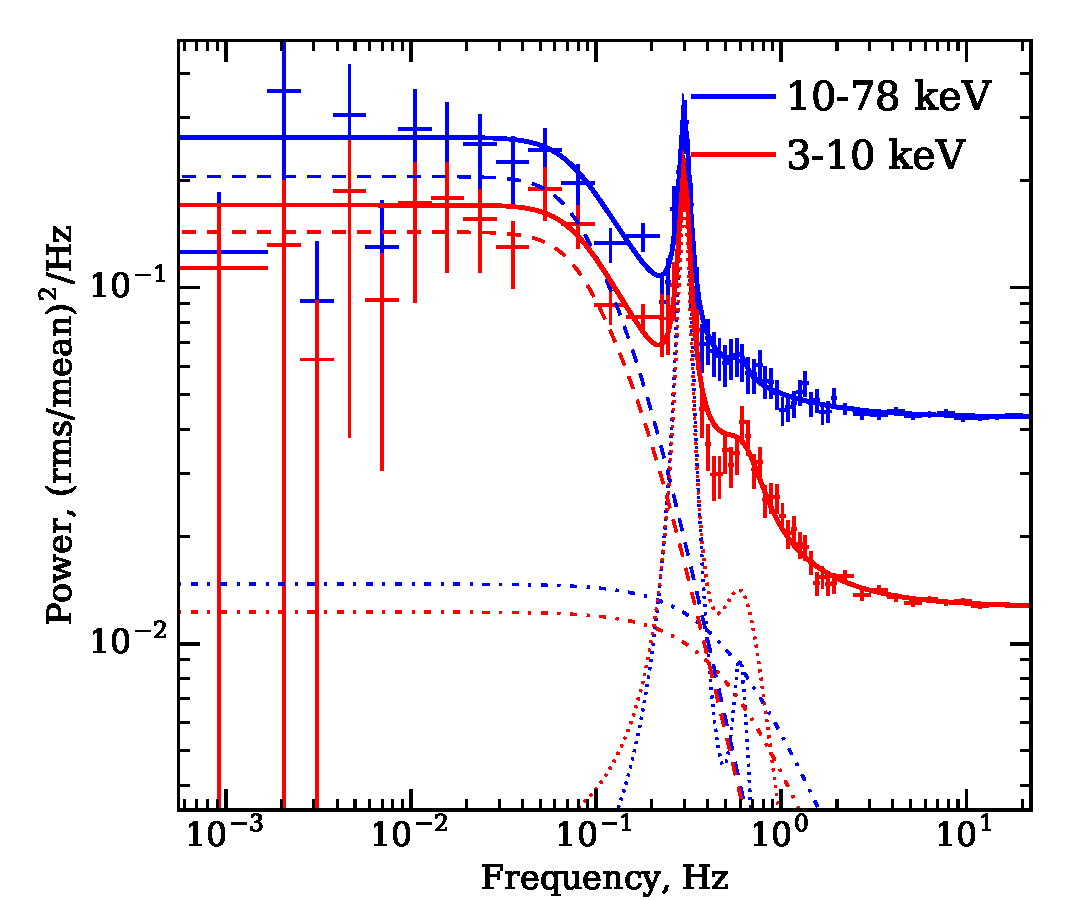
\includegraphics[width=0.5\columnwidth]{NuFirst.pdf}
        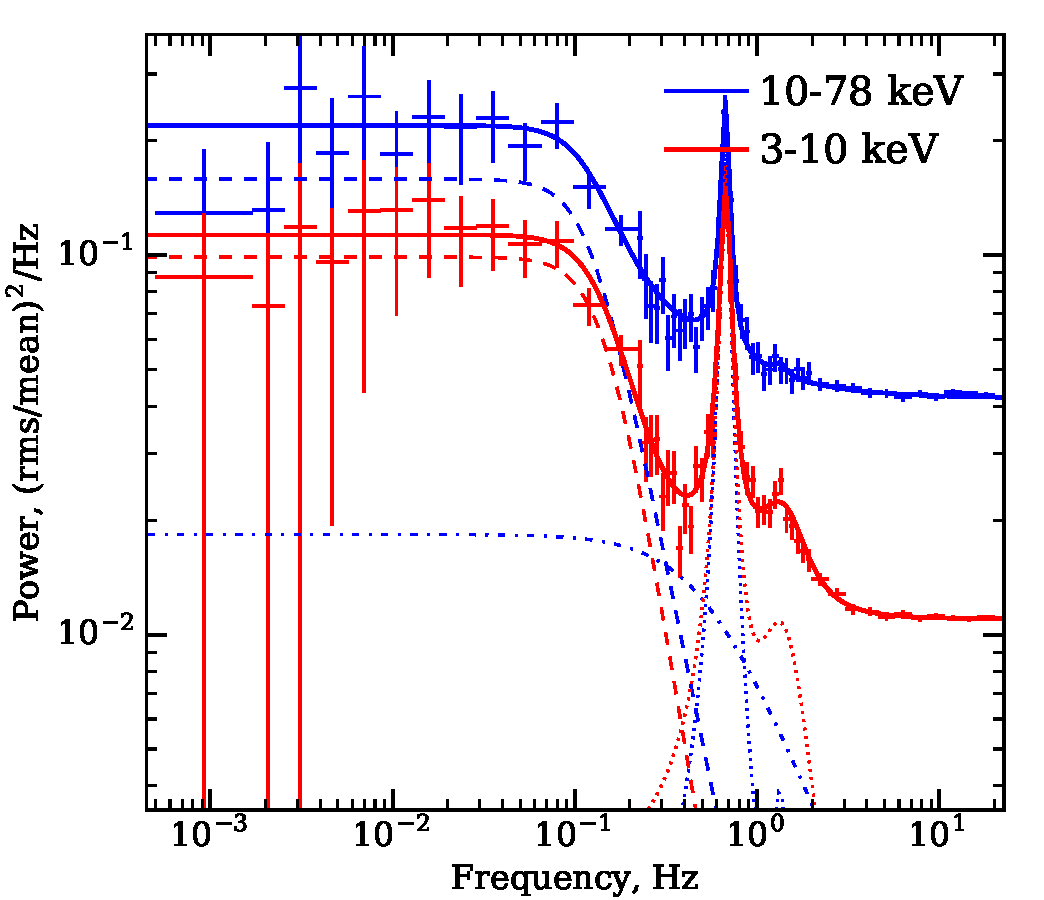
\includegraphics[width=0.5\columnwidth]{NuLast.pdf}
        \caption{On the left panel power spectra obtained in the soft (red) and hard (black) bands at the beginning of {\it NuSTAR} observation. 
        On the right column same spectra obtained at the end of the observation.}
        \label{fig:ps_example}
\end{figure}

In Table \ref{tbl:ps_fit_parameters} one can fined obtained fit parameters for the 13 separate uninterrupted {\it NuSTAR} time series.

\subsection{Coherence}

    Power spectra of XBs are often have a complex shape with broad band noise and QPO like features, and numerous different models of these system were suggested to explain each particular feature. 
\citep{vaughan97} suggested to use coherence between different energy bands in order to obtain additional information on the source time properties. 
They define coherence as 
\begin{equation}
    C(f) = \frac{|<H(f)>^*<S(f)>|^2}{<|H(f)|^2><|S(f)|^2>}
    \label{eq:nowak_coh}
\end{equation}
where $H(f)$ and $S(f)$ are Fourier function of time series in hard and soft bands correspondingly. 
This function demonstrates the similarity of stochastic time signal in both bands. 
Different models of the XBs variability formation suggest that the signal in two energy bands can be partially independent, while the shape of the power spectra is conserved.
It appears that in many sources coherence between soft and hard X-ray bands is close to unity \citep{nowak99, wijnands01, eijden17}, in contrary to different models predictions \citep[see, discussion in][]{vaughan97}.

Following method \citep{nowak99} we estimated correlation of \grs\ light-curves obtained in the soft and hard energy bands. 
Since for the timing analysis we use {\it NuSTAR} data, we adopt following energy bands for the soft and hard light-curves correspondingly: 3--10~keV (soft) and 10--79~keV (hard).

In contrast to the \citep{nowak99} study, net count rate, obtained in \grs\ {\it NuSTAR} observation is {\bf 160~s$^{-1}$}, it follows that approximately quarter of the total variability power is due to the Poisson noise. 
As was discussed in \citep{nowak99} the correlation of two independent time series demonstrates large errors on the frequencies dominated with Poisson noise, due to the random walk in the 2-D complex space.
We also found, that the correlation of the light-curves obtained from {\it NuSTAR} is subjected by the dead-time and crosstalk effects between the energy bands.
In order to eliminate this effects, following the recipe suggested in \cite{2015ApJ...800..109B} for power spectra estimation, we find crossproducts of the light-curves Fourier functions obtained on the different modules - e.g. correlations of the light-curve obtained in the soft band on the FPMA module with the light-curve in the hard band obtained in the FPMB and vice versa.
Obtained correlation does not contain polluting signal from the blocking dead time. 

After that, as explained in \citep{Nowak99}, one should find the amplitude of the fully coherent signal $<|H(f)|^2><|S(f)|^2>$ in order to estimate coherence of the signals. 
There is several different options, which one can be use to estimate this normalization:
\begin{itemize}
        \item Use observed of the power spectra in each energy band. 
                The drawback of this method is that power spectra contain Poisson noise component constant on all frequencies and dominating over the source variability on high frequencies. 
                Thus, since Poisson noise is not coherent,  if one use this normalization as a denominator in Eq.~\ref{eq:nowak_coh} coherence estimation will be dumped on the value equal to the ratio of the Poisson noise to the source signal power on each frequency.
        \item Instead of the observed power spectra, one can use approximation of the power spectra with analytical models. 
                Poisson noise component can be discarded in analytical model, thus only source signal is conserved. 
                The drawback is that due to the Dead time effects Poisson noise has a complex form and can not be easily estimated with simple model.
        \item Use coherent part of the Fourier function of light curves in two modules \citep{2015ApJ...800..109B} or it's approximation with the analytical function. 
                It should be noted, that obtained coherent part of the ${\rm re}(H_{\rm A}(f)^*H_{\rm B}(f))$ has complex statistic which not restricting negative values, which must be ignored or modified thus affecting result.  
                We also found, that for short time series, one should use more complex likelihood criterion in order to fit coherent signal with analytical functions, since the statistic is still far from Gaussian and obtained fits are often unstable.
\end{itemize}

\begin{figure}
    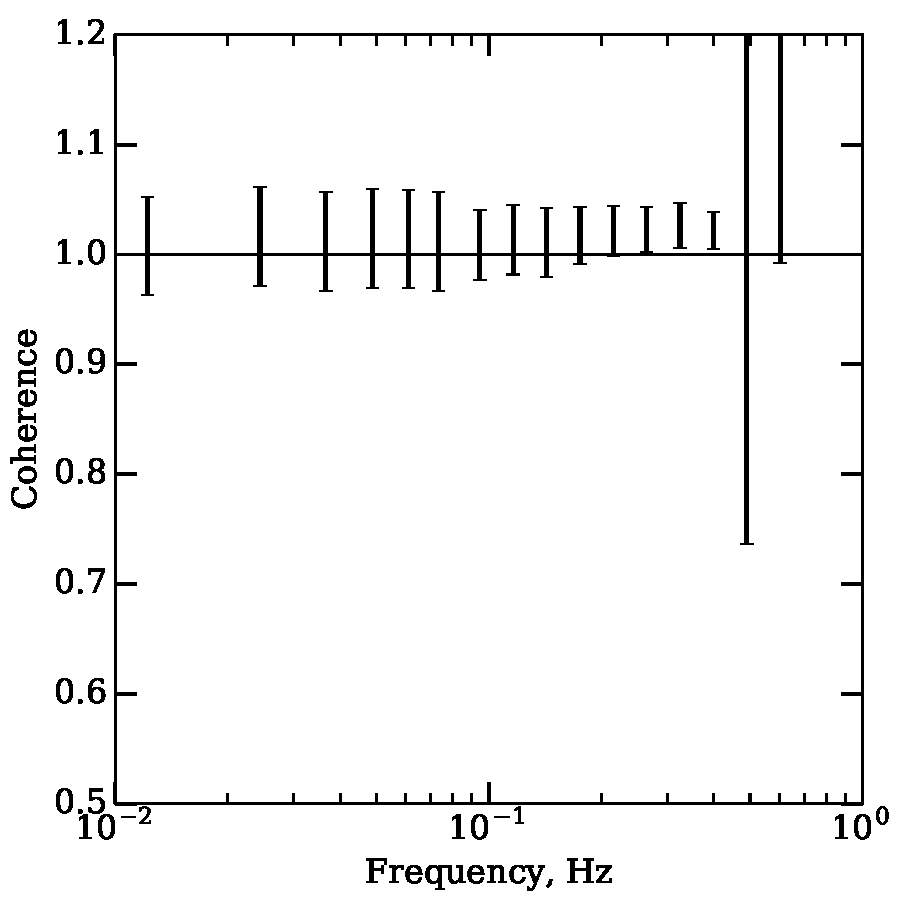
\includegraphics[width=\columnwidth]{coherence_grs.pdf}
    \caption{Coherence between the soft (3--10~keV) and hard (10--78~keV) energy bands as a function of frequency} 
    \label{fig:coherence}
\end{figure}


On Figure~\ref{fig:coherence} presented measured coherence between hard and soft band on the frequencies up to $\sim1$~Hz. 
The coherence was obtained with the third method with negative values discarded. 
%This method allows to rid out of the complex high frequency features connected with the cross-talk in the energy bands and blocking dead time effects.

%There is a drawback with this method, 
%Since Poisson noise in the two considered energy bands is independent, correlation of the light-curves computed with the eq.4 from \cite{Nowak99} is dumped, and tends to zero on the frequencies where Poisson noise dominates over the source variability.
%Therefore, to obtain proper estimates on the correlation function and phase lags between soft and hard flux, instead of the product of estimates of power spectra in two energy bands as denominator we are use analytical model $P_{h}(f)\cdotP_{s}(f)$ describing corresponding power spectra. 
%Here $P_h(f)$ and $P_s(f)$ - analytical function, approximating the power spectra in soft and hard bands.
%We found, that the power spectra in this bands are very similar to each other and can be fitted on the frequencies above 0.01~Hz with the following function:


%We found, that our estimate on the coherence, growths significantly on the frequencies above $\sim2$~Hz, where Poisson noise begins to dominate over the source intrinsic variability.
%This can be explained with the uncertainty of the obtained model parameters or its simplicity. 
%We found that for both soft and hard bands, obtained fits suggest very abrupt drop in power between the QPO and low-frequency plateau, it leads to very steep index of the power-law component. 
%Therefore growth of the coherence estimates on the higher frequencies is due to the underestimation of the source intrinsic variability on the corresponding frequencies.

%We found, that, similarly to different XBs, light curves in the hard and soft bands demonstrate strong correlation up to the high frequencies, however, we were not able to estimate properly coherence above 2~Hz due to the Poisson noise.

\subsection{Phase lags}
    Most of the models of the accretion flow which describe variability and energy spectra formation, suggest the time lag between the fluxes in different energy bands. 
For example in some models of the energy spectra formation, time lag is naturally arise due to the geometry of the corona and properties of the inverse Comptonization process \citep[see, e.g.][]{kotov01}.
Phase lag is also suggested from the propagating fluctuations model - hard photons are emitted from the inner parts of the accretion flow and perturbations spend some time before reaching them. 

It also was found, that phase lag of XBs, probably depends on the system inclination angle \citep{eijeden17}, it also definitely contain information about the characteristic times of the system, and therefore can be proxy to the compact object mass \citep{}. 

Phase lags can be estimated as a product of the mean phase of the set of Fourier spectra and the corresponding frequency:
$$<F_h(f)F_s(f)> = n(f)e^{-i\phi(f)}$$ 
here, $F_h(f)$ and $F_s(f)$ are Fourier functions of the light-curves in the hard and soft bands, $\phi(f)$ is the phase lag and $$n(f)$$ - is the square root of the power spectrum of the soft and hard light-curves coherent part. 

To estimate phase lags we use the same approach as for the coherence.



We found that the total power in the second QPO harmonic in the soft band is comparable to the total power in the main harmonic, in the hard band second harmonic is $\approx3$ times less powerfull than the main. 
Total power of the harmonics growing with the source count-rate and QPO frequency in the soft and hard energy bands (see Table~\ref{tab:timing}). 
If the QPO has geometrical origin - i.e. it's due to the change of the view on the some statical illumination pattern like in the \citep{IVK09} model, than this pattern is more complex in the soft energy band. 

%If the QPO is due to the changing of our field of view on some static pattern, like in the \citep{ivk09} model, than it follows that QPOs in this bands have different origin - i.e. QPO in the soft band is due to the scattering of the photones from precessing corona, while QPOs  reflection of the ro

